\documentclass[dvipsnames,beamer,10pt]{standalone}

\usepackage{tikz}
\usepackage{arrayjob}




\usetikzlibrary{positioning,decorations.pathreplacing,fit}
\usetikzlibrary{decorations.markings,arrows.meta,shapes.arrows,arrows}
\usetikzlibrary{bending}
\usetikzlibrary{calc}

\definecolor{mygreen}{RGB}{0,128,80}
\colorlet{darkgreen}{mygreen!90!black}

\providecommand{\adlog}{\textcolor{red}{a}}
\providecommand{\bdlog}{\textcolor{blue}{b}}
\providecommand{\cdlog}{\textcolor{Plum}{c}}
\providecommand{\ddlog}{\textcolor{OliveGreen}{d}}
\providecommand{\dlog}[2]{\textcolor{#1}{#2}}
\providecommand{\ua}[1]{\dlog{red}{#1}}
\providecommand{\ub}[1]{\dlog{blue}{#1}}
\providecommand{\uc}[1]{\dlog{Plum}{#1}}
\providecommand{\ud}[1]{\dlog{OliveGreen}{#1}}

%\DeclareMathSizes{10.0}{12}{5}{4}


\begin{document}




\begin{standaloneframe}

\resizebox{1\textwidth}{!}{



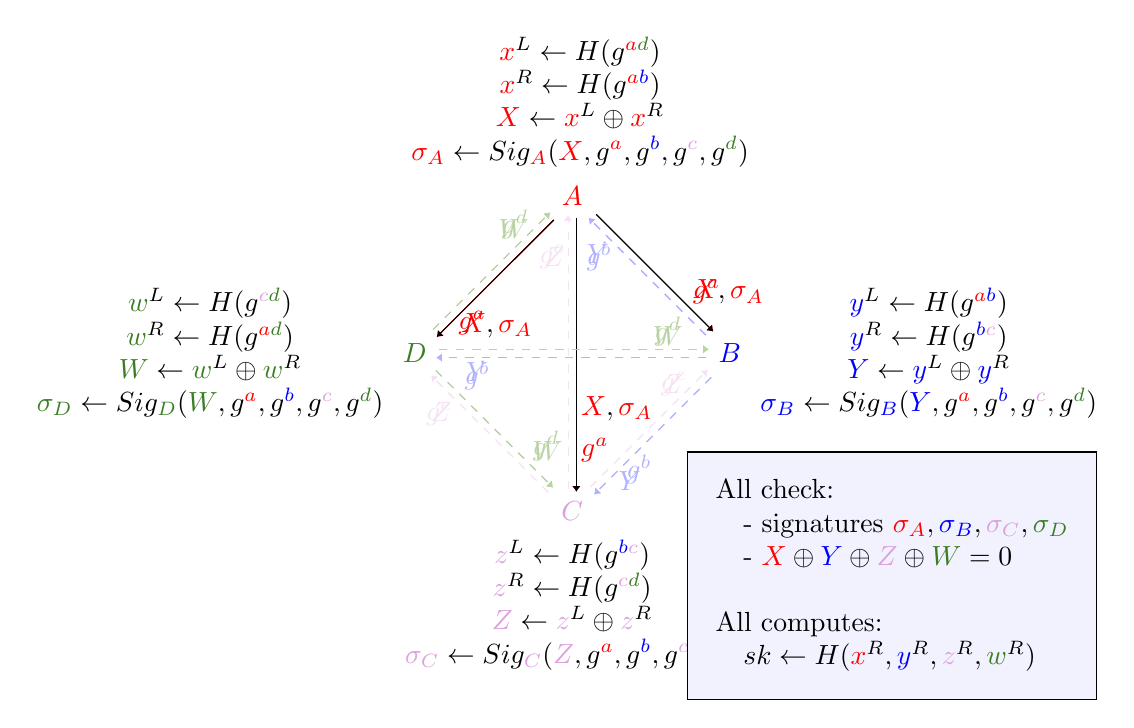
\begin{tikzpicture}[
		mycircle/.style= {fill,circle, inner sep=1pt},
		DHshare/.style= {inner sep=-1pt,pos=0.7},
		>={Latex[length=2pt,width=3pt]},<->,shorten <= 1pt,
		main node/.style={},		
	]
		

	\newcommand*{\MainNum}{4}
	\newcommand*{\MainRadius}{2cm} 
	\newcommand*{\MainStartAngle}{180}
	\newcommand*{\MainBend}{35}
	
	% Print main nodes, node names: p1, p2, ...
	\coordinate (M) at (0,0);

		 
	\node (u1) at ({-1*360/\MainNum + \MainStartAngle}:\MainRadius) {\textcolor{red}{$A$}};
	\node[inner sep=1pt] (m_1) at ({-1*360/\MainNum + 135}:\MainRadius + 0.4cm) {};
	
	\node (u2) at ({-2*360/\MainNum + \MainStartAngle}:\MainRadius) {\textcolor{blue}{$B$}};
	\node[inner sep=1pt] (m_2) at ({-2*360/\MainNum + 135}:\MainRadius + 0.4cm) {};
	
	\node (u3) at ({-3*360/\MainNum + \MainStartAngle}:\MainRadius) {\textcolor{Plum}{$C$}};
	\node[inner sep=1pt] (m_3) at ({-3*360/\MainNum + 135}:\MainRadius + 0.4cm) {};
	
	\node (u4) at ({-4*360/\MainNum + \MainStartAngle}:\MainRadius) {\textcolor{OliveGreen}{$D$}};
	\node[inner sep=1pt] (m_4) at ({-4*360/\MainNum + 135}:\MainRadius + 0.4cm) {};

	\uncover<+-+(1)>{
		\draw[->,red,transform canvas={xshift=1pt,yshift=1pt}] (u1) -- node[above right,pos=0.8,inner sep=1pt] {$g^{\adlog}$} (u2); 
		\draw[->,red,transform canvas={xshift=1.5pt}] (u1) -- node[right,inner sep=1.5pt,pos=0.85] {$g^{\adlog}$} (u3); 
		\draw[->,red,transform canvas={xshift=1pt,yshift=-1pt}] (u1) -- node[below right,pos=0.8,inner sep=-1pt] {$g^{\adlog}$} (u4); 
	
		\draw[->,dashed,blue!30,transform canvas={xshift=-1pt,yshift=-1pt}] (u2) -- node[below left,inner sep=0, pos=0.8] {$g^{b}$} (u1); 
		\draw[->,dashed,blue!30,transform canvas={xshift=1pt,yshift=-1pt}] (u2) -- node[below right,inner sep=-1.5pt,pos=0.7] {$g^{b}$} (u3); 
		\draw[->,dashed,blue!30,transform canvas={yshift=-1.5pt}] (u2) -- node[below,inner sep=1pt,pos=0.85] {$g^{b}$} (u4);
		
		\draw[->,dashed,Plum!30,transform canvas={xshift=-1.5pt}] (u3) -- node[left,inner sep=1pt,pos=0.85] {$g^{c}$} (u1); 
		\draw[->,dashed,Plum!30,transform canvas={xshift=-1pt,yshift=1pt}] (u3) -- node[above left,inner sep=-1pt,pos=0.8] {$g^{c}$} (u2); 
		\draw[->,dashed,Plum!30,transform canvas={xshift=-1pt,yshift=-1pt}] (u3) -- node[below left,inner sep=1pt,pos=0.8] {$g^{c}$} (u4);
		
		\draw[->,dashed,OliveGreen!30,transform canvas={xshift=-1pt,yshift=1pt}] (u4) -- node[above left,inner sep=-1pt, pos=0.8] {$g^{d}$} (u1); 
		\draw[->,dashed,OliveGreen!30,transform canvas={yshift=1.5pt}] (u4) -- node[above,inner sep=1pt,pos=0.85] {$g^{d}$} (u2); 
		\draw[->,dashed,OliveGreen!30,transform canvas={yshift=1.5pt}] (u4) -- node[above right,inner sep=1pt,pos=0.8] {$g^{d}$} (u3);		 	 
	}
	
	
	\uncover<+->{
		\node[above =0 of u1,align=center,xshift=0.1cm] (X) {
			$\ua{x}^L \gets H(g^{\adlog\ddlog})$\\
			$\ua{x}^R \gets H(g^{\adlog\bdlog})$\\
			$\ua{X} \gets \ua{x}^L \oplus \ua{x}^R$\\
			$\ua{\sigma_A} \gets Sig_{\ua{A}}(\ua{X}, g^{\adlog},g^{\bdlog},g^{\cdlog},g^{\ddlog})$
		};
	}
		
	
	\uncover<+->{
		\draw[->,transform canvas={xshift=1pt,yshift=1pt}] (u1) -- node[above right,pos=0.8,inner sep=1pt] {$\ua{X}, \ua{\sigma_A}$} (u2); 
		\draw[->,transform canvas={xshift=1.5pt}] (u1) -- node[right,inner sep=1.5pt,pos=0.7] {$\ua{X}, \ua{\sigma_A}$} (u3); 
		\draw[->,transform canvas={xshift=1pt,yshift=-1pt}] (u1) -- node[below right,pos=0.8,inner sep=0pt] {$\ua{X}, \ua{\sigma_A}$} (u4); 
	}
	

	
	
	\uncover<+->{	
		\draw[->,dashed,blue!30,transform canvas={xshift=-1pt,yshift=-1pt}] (u2) -- node[below left,inner sep=1, pos=0.8] {$\dlog{blue!30}{Y}$} (u1); 
		\draw[->,dashed,blue!30,transform canvas={xshift=1pt,yshift=-1pt}] (u2) -- node[below right,inner sep=0pt,pos=0.8] {$\dlog{blue!30}{Y}$} (u3); 
		\draw[->,dashed,blue!30,transform canvas={yshift=-1.5pt}] (u2) -- node[below,inner sep=1.5pt,pos=0.85] {$\dlog{blue!30}{Y}$} (u4);
		
		\draw[->,dashed,Plum!30,transform canvas={xshift=-1.5pt}] (u3) -- node[left,inner sep=1pt,pos=0.85] {$\dlog{Plum!30}{Z}$} (u1); 
		\draw[->,dashed,Plum!30,transform canvas={xshift=-1pt,yshift=1pt}] (u3) -- node[above left,inner sep=0pt,pos=0.8] {$\dlog{Plum!30}{Z}$} (u2); 
		\draw[->,dashed,Plum!30,transform canvas={xshift=-1pt,yshift=-1pt}] (u3) -- node[below left,inner sep=1pt,pos=0.8] {$\dlog{Plum!30}{Z}$} (u4);
		
		\draw[->,dashed,OliveGreen!30,transform canvas={xshift=-1pt,yshift=1pt}] (u4) -- node[above left,inner sep=-1pt, pos=0.8] {$\dlog{OliveGreen!30}{W}$} (u1); 
		\draw[->,dashed,OliveGreen!30,transform canvas={yshift=1.5pt}] (u4) -- node[above,inner sep=1pt,pos=0.85] {$\dlog{OliveGreen!30}{W}$} (u2); 
		\draw[->,dashed,OliveGreen!30,transform canvas={yshift=1.5pt}] (u4) -- node[above right,inner sep=1pt,pos=0.8] {$\dlog{OliveGreen!30}{W}$} (u3);	
		
		\node[right =0 of u2,align=center] (Y) {
			$\ub{y}^L \gets H(g^{\adlog\bdlog})$\\
			$\ub{y}^R \gets H(g^{\bdlog\cdlog})$\\
			$\ub{Y} \gets \ub{y}^L \oplus \ub{y}^R$\\
			$\ub{\sigma_B} \gets Sig_{\ub{B}}(\ub{Y}, g^{\adlog},g^{\bdlog},g^{\cdlog},g^{\ddlog})$
		};
		\node[below =0 of u3,align=center] (Z) {
			$\uc{z}^L \gets H(g^{\bdlog\cdlog})$\\
			$\uc{z}^R \gets H(g^{\cdlog\ddlog})$\\
			$\uc{Z} \gets \uc{z}^L \oplus \uc{z}^R$\\
			$\uc{\sigma_C} \gets Sig_{\uc{C}}(\uc{Z}, g^{\adlog},g^{\bdlog},g^{\cdlog},g^{\ddlog})$
		};
		\node[left =0 of u4,align=center] (W) {
			$\ud{w}^L \gets H(g^{\cdlog\ddlog})$\\
			$\ud{w}^R \gets H(g^{\adlog\ddlog})$\\
			$\ud{W} \gets \ud{w}^L \oplus \ud{w}^R$\\
			$\ud{\sigma_D} \gets Sig_{\ud{D}}(\ud{W}, g^{\adlog},g^{\bdlog},g^{\cdlog},g^{\ddlog})$
		};		 	 
	}

	
	\uncover<+->{
		\node[below right=-1cm and 1.2cm of u3,draw,fill=blue!5,align=left,inner sep=10pt] {
			All check:\\
				$\quad$- signatures $\ua{\sigma_A}, \ub{\sigma_B}, \uc{\sigma_C}, \ud{\sigma_D}$  \\
				$\quad$- $\ua{X} \oplus \ub{Y} \oplus \uc{Z} \oplus \ud{W} = 0$\\
				\\
			All computes:\\
				$\quad$$sk \gets H(\ua{x}^R, \ub{y}^R, \uc{z}^R, \ud{w}^R)$
		};
	}

\end{tikzpicture}


}
\end{standaloneframe}


\end{document}